\chapter{Problem Statement and Motivation}

The entry point to research in this area was asking the question: ``How does the software managing critical infrastructure, like FREEDM, behave when a critical component, the communication infrastructure, is not operating correctly?'' 
Historically, leader elections have had limited applications in critical systems. However, in the smart-grid domain, there is a great opportunity to apply leader election algorithms in a directly beneficial way. \cite{LOADBALANCING} presents a simple scheme for performing power distribution and stabilization that relies on formed groups. Algorithms like Incremental Consensus Algorithm\cite{INCREMENTALCONSENSUS}, begin with the assumption that there is a group of processes who coordinate to distribute power. In a system where 100\% up time is not guaranteed, leader elections are a promising method of establishing these groups.
A strong cyber-physical system should be able to survive and adapt to network outages in both the physical and cyber domains. When one of these outages occurs, the physical or cyber components must take corrective action to allow the rest of the network to continue operating normally.

This work observes the effects of message omission on the group management module of the Distributed Grid Intelligence (DGI) used by the FREEDM smart-grid project. This system uses a broker system architecture to coordinate several software modules that form a control system for a smart power grid. These modules include: group management, which handles coordinating processes via leader election; state collection, a module which
captures a global system state; and load balancing, which uses the captured global state to bring the system to a stable state.

It is important for the designer of a cyber-physical system to consider what effects the cyber components will have on the overall system. Failures in the cyber domain can lead to critical instabilities which bring down the entire system if not handled properly.  In fact, there is a major shortage of work within the realm of the effects cyber outages have on \ac{CPS}\cite{CYBERRESEARCHCALL}\cite{SMARTGRIDBENEFITS}.
The analysis presented in this work focuses on quantifiable changes in the amount of time a \ac{DGI} could spend participating in energy management with other processes.

Using the DGI as a starting point, the analysis of the leader election algorithm in the DGI began with analysis of its behavior when messages were lost.
To do this, the DGI software was subjected to omission faults while the state of the algorithm was captured over a period of examination.
The goal of these experiments was to examine what behavior the DGI would exhibit during the fault conditions.
Additionally, we hoped to determine the advantages and disadvantages of using a more complicated, reliable message retransmission protocol over a more simple one without retransmission.

\section{INITIAL EXPERIMENTS}

The initial experiments were collected from a non-real time version of the DGI code.
Experiments measured the \ac{IGT}, a measure of availability, for various sets of DGI running the leader election algorithm during omission fault conditions.
Additionally, the experiments examined two communication modes, the Sequenced Reliable Connection, and the Sequenced Unreliable Connection.
Both methods of communication were valid approaches for the message passing requirements of the DGI.

\subsection{Sequenced Reliable Connection (SRC)}

The \ac{SRC} is a modified send and wait protocol with the ability to stop resending messages and move on to the next one in the queue if the message delivery time is too long. When designing this scheme we wanted to achieve several criteria:

\begin{itemize}
\item Messages must be accepted in order - Some distributed algorithms rely on the assumption that the underlying message channel is FIFO.
\item Messages can become irrelevant - Some messages may only have a short period in which they are worth sending. Outside of that time period, they should be considered inconsequential and should be skipped. To achieve this, we have added message expiration times. After a specified amount of time has passed, the sender will no longer attempt to write that message to the channel. Instead, it will proceed to the next unexpired message and attach a ``kill'' value to the message being sent, with the number of the last message the sender knows the receiver accepted.
\item As much effort as possible should be applied to deliver a message while it is still relevant.
\end{itemize}

There was one adjustable parameter, the resend time, which controls how often the system would attempt to deliver a message it had not yet received an acknowledgment for.

\subsection{Sequenced Unreliable Connection (SUC)}

The \ac{SUC} protocol is simply a best effort protocol: it employs a sliding window to try to deliver messages as quickly as possible.
The receiver will look for increasing sequence numbers and disregard any message that is of a lower sequence number than is expected. The purpose of this protocol is to implement a bare minimum: messages are accepted in the order they are sent.

Like the \ac{SRC} protocol, the SUC protocol's resend time can be adjusted. Additionally, the window size is configurable, but was left unchanged for the tests presented in this work.

\section{INITIAL RESULTS}

The collected results from the tests were divided into several target scenarios as well as the protocol used.

The first minute of each test in the experimental test was discarded so that any transients in the test could be removed.
The tests were run for ten minutes, however the maximum result was 9 minutes of \ac{IGT}.
These graphs first appeared in \cite{CRITIS2012}.

\subsection{Sequenced Reliable Connection, Two Process Case}


The 100ms resend SRC test with two processes was considered a type of control in this study.
These tests, pictured in Figure \ref{fig:IGT-SRC-2NODE-100}, highlighted the availability of the DGI with the SRC protocol.
The maximum \ac{IGT} of 9 minutes was achieved with only 15\% of datagrams arriving at the receiver. 

Figure \ref{fig:IGT-SRC-2NODE-200} demonstrates that as the rate at which lost datagrams were re-sent was decreased to 200ms, the in-group time decreased.
This behavior was expected.
Each exchange had a time limit for each message to arrive and the number of attempts was reduced by increasing the resend time.

\begin{figure}[htbp]
    \centering
    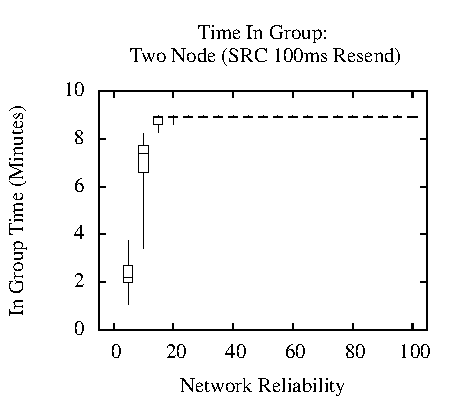
\includegraphics[width=0.75\textwidth]{2NODE-SRC-100-GROUP.pdf}
    \caption{\ac{IGT} over a 10 minute run for a two process system with a 100ms resend time.}
    \label{fig:IGT-SRC-2NODE-100}
\end{figure}

\begin{figure}[htbp]
    \centering
    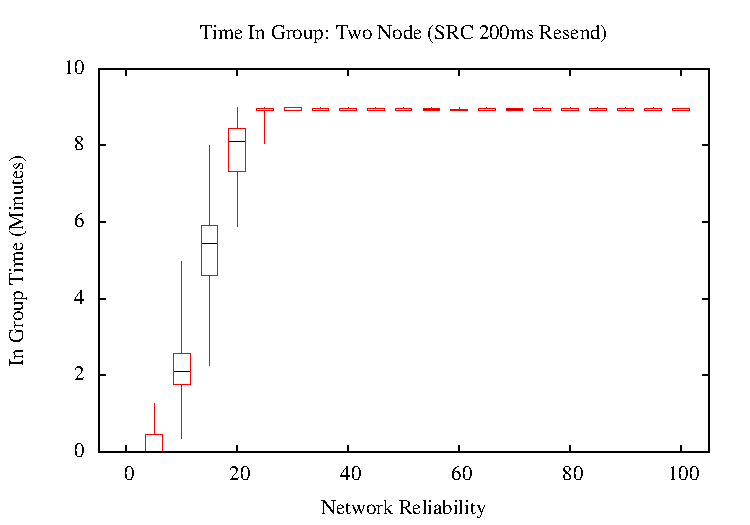
\includegraphics[width=0.75\textwidth]{2NODE-SRC-200-GROUP.pdf}
    \caption{\ac{IGT} over a 10 minute run for a two process system with a 200ms resend time.}
    \label{fig:IGT-SRC-2NODE-200}
\end{figure}

\subsection{Sequenced Reliable Connection, Transient Partition Case}


The transient partition case was a simple example in which a network partition separates two groups of DGI processes.
In the simplest case, where the opposite side of the partition was unreachable, processes formed a group with the other processes on the same side of the partition.
Two processes were present on each side of the partition.
The 100ms case is shown in Figures \ref{fig:MGS-SRC-TRANS-100} and \ref{fig:IGT-SRC-TRANS-100}.

While messages could not cross the partition, the DGIs stay in a group with the processes on the same side of the partition, leading to an in-group time of 9 minutes (the maximum value possible).
As packets began to cross the partition (as the omission probability decreased), DGI instances on either side attempted to complete elections with the processes on the opposite partition and the in group time began to decrease.
During this time, however, the mean group size continued to increase.
Thus, while the elections were decreasing the amount of time that the module spent in a state where it can actively do work, it typically did not fall into a state where it was in a group by itself. 
As result, most of the lost \ac{IGT} came from elections.
\begin{figure}[htbp]
    \centering
    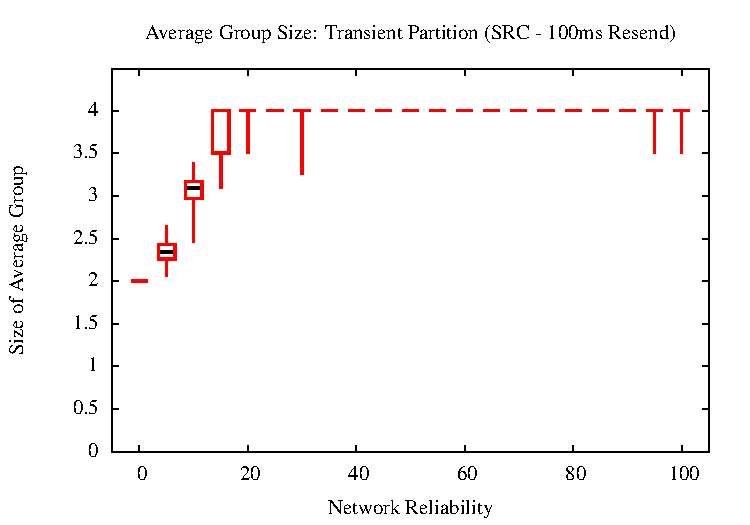
\includegraphics[width=0.75\textwidth]{TRANS-SRC-100-SIZE.pdf}
    \caption{Average size of formed groups for the transient partition case with a 100ms resend time.}
    \label{fig:MGS-SRC-TRANS-100}
\end{figure}%
\begin{figure}[htbp]
    \centering
    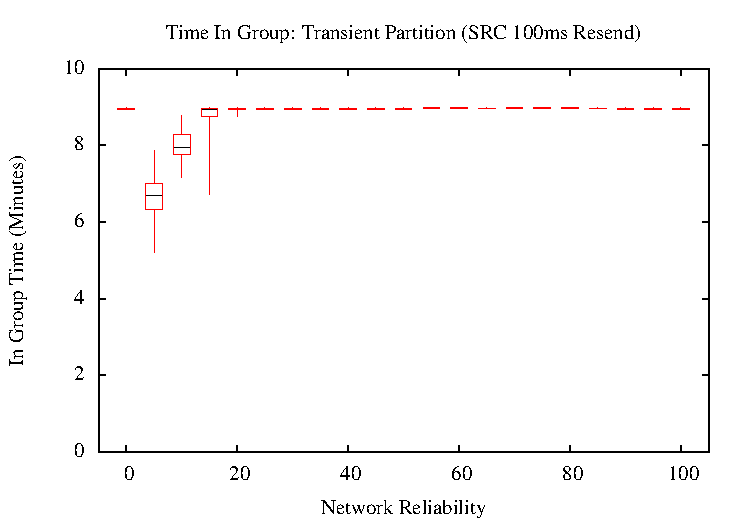
\includegraphics[width=0.75\textwidth]{TRANS-SRC-100-GROUP.pdf}
    \caption{\ac{IGT} over a 10 minute run for the transient partition case with a 100ms resend time.}
    \label{fig:IGT-SRC-TRANS-100}
\end{figure}

The 200ms case (illustrated in Figures \ref{fig:MGS-SRC-TRANS-200} and \ref{fig:IGT-SRC-TRANS-200}) suggests a similar behavior to Figures \ref{fig:MGS-SRC-TRANS-100} and \ref{fig:IGT-SRC-TRANS-100}, with a wider valley produced by the reduced number of datagrams.
The mean group size dipped below two in Figure \ref{fig:MGS-SRC-TRANS-200}, possibly because longer resend times allowed for a greater number race conditions between potential leaders.
The race conditions are discussed during the SUC section since it was more prevalent in those experiments.

\begin{figure}[htbp]
\centering
    \centering
    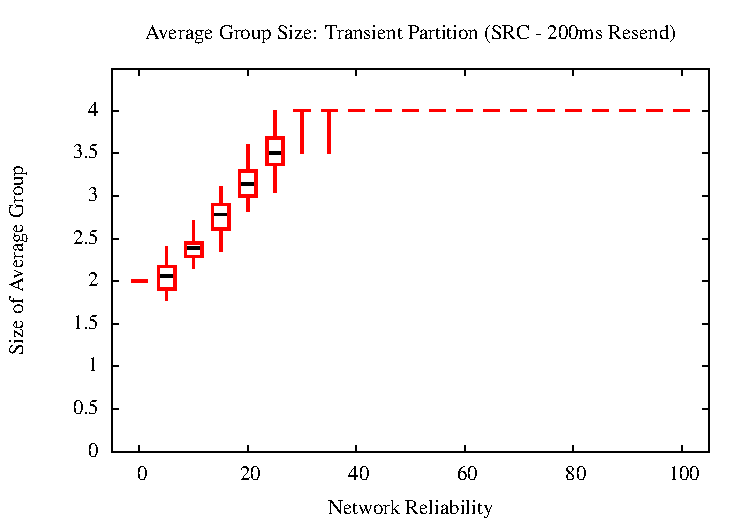
\includegraphics[width=0.75\textwidth]{TRANS-SRC-200-SIZE.pdf}
    \caption{Average size of formed groups for the transient partition case with a 200ms resend time.}
    \label{fig:MGS-SRC-TRANS-200}
\end{figure}
\begin{figure}[htbp]
    \centering
    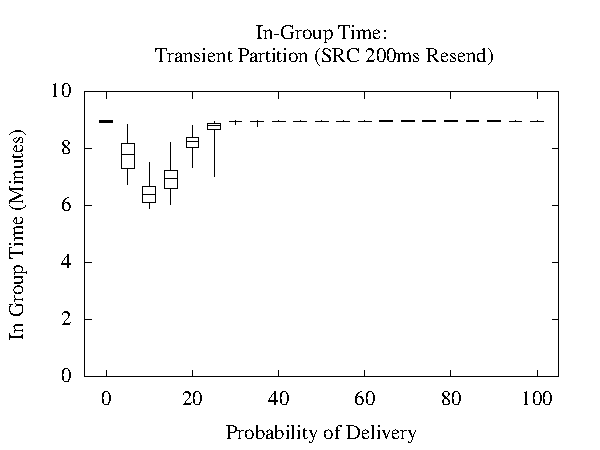
\includegraphics[width=0.75\textwidth]{TRANS-SRC-200-GROUP.pdf}
    \caption{\ac{IGT} over a 10 minute run for the transient partition case with a 200ms resend time.}
    \label{fig:IGT-SRC-TRANS-200}
\end{figure}

\subsection{Sequenced Unreliable Connection, Two Process Case}

The SUC protocol's experimental tests revealed an immediate problem.
There was a general increasing trend for the amount of \ac{IGT}, shown in Figure \ref{fig:IGT-SUC-2NODE-100}.
However, there was a high amount of variance for every trial.

In the 200ms resend case (illustrated in Figure \ref{fig:IGT-SUC-2NODE-200}), a greater growth rate occurred in the \ac{IGT} as the omission probability decreased.
When an average was taken across all of the collected data points from the experiment, the average \ac{IGT} is higher for the 200ms case than it was for the 100ms case (6.86 minutes vs 6.09 minutes).
There was a large amount of variance in the collected \ac{IGT}, however.
As a result, it is not possible to state with confidence that the there is a significant difference between the two cases.

\begin{figure}[htbp]
    \centering
    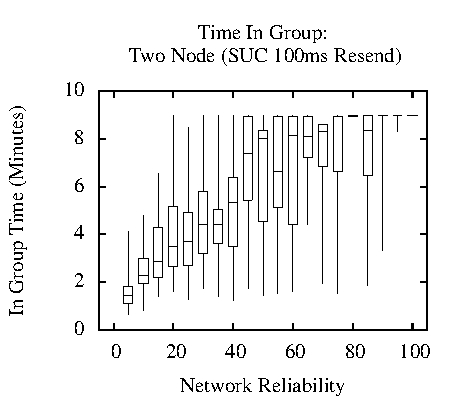
\includegraphics[width=0.75\textwidth]{2NODE-SUC-100-GROUP.pdf}
    \caption{\ac{IGT} over a 10 minute run for two process system with 100ms resend time.}
    \label{fig:IGT-SUC-2NODE-100}
\end{figure}%
\begin{figure}[htbp]
    \centering
    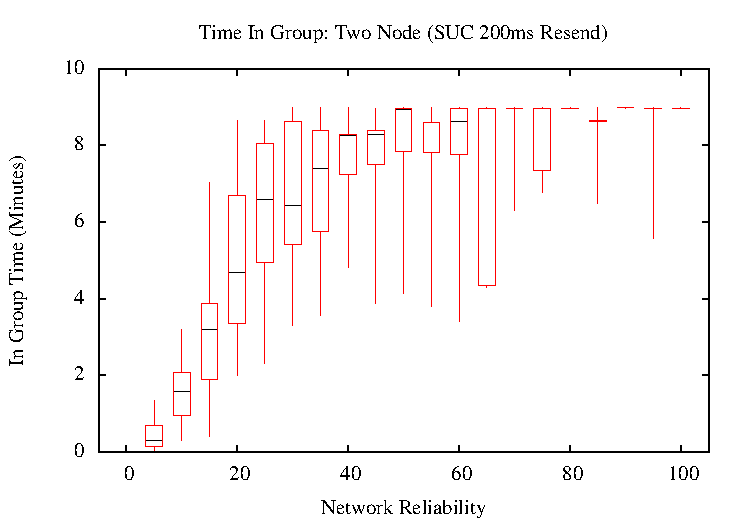
\includegraphics[width=0.75\textwidth]{2NODE-SUC-200-GROUP.pdf}
    \caption{\ac{IGT} over a 10 minute run for two process system with 200ms resend time.}
    \label{fig:IGT-SUC-2NODE-200}
\end{figure}

\section{MARKOV MODELS}

After collecting the results from the initial experiments, we sought to describe the observed behavior through the use of continuous-time Markov chains.
The behavior of the DGI transition between various states of grouping was calibrated with initial results and applied to other scenarios to validate the results.
This approach had several shortcomings.
First, for reasons we will demonstrate in subsequent chapters, the leader election algorithm modeled in these chains was not memoryless: the state used in the Markov chain was not sufficient to capture the interaction between processes that was occurring.
Secondly, the continuous time model could not accurately capture the execution model of the DGI.
In the DGI, processes synchronize with each other to execute in a partially-synchronous manner.
As a result, the execution and transition between states is more accurately described with a discrete-time Markov chain.

The presented methodology of constructing the model was initially calibrated against the original two-process case.
This calibration used a non-real-time version of the DGI code.
The resulting Markov chain was processed using SharpE\cite{SHARPE}\cite{SHARPE2}, a popular tool for reliability analysis.
SharpE measured the reward collected in 600 seconds, minus the reward that was collected in the first 60 seconds. 
Discarding the reward from the first 60 seconds emulated the 60 seconds that were discarded in the experimental runs.
The SharpE results are plotted along with the experimental results in Figures \ref{fig:COMPARE-SUC-2NODE-100} and \ref{fig:COMPARE-SUC-2NODE-200}.

\begin{figure}[htbp]
    \centering
    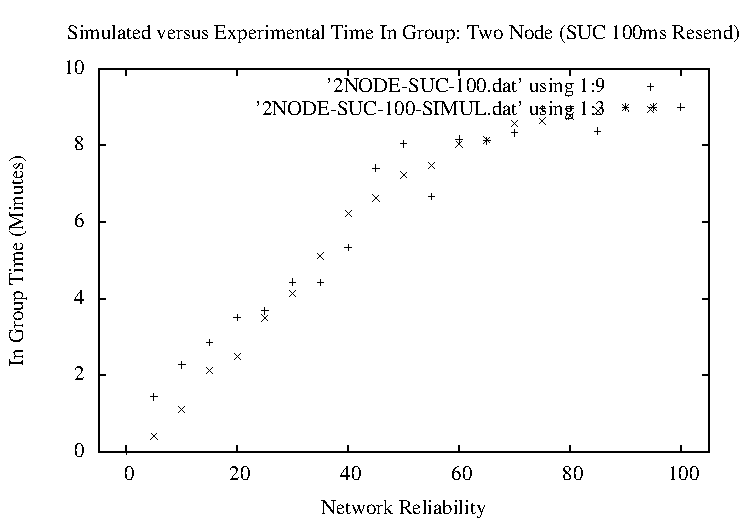
\includegraphics[width=0.75\textwidth]{2NODE-SUC-100-COMPARE.pdf}
    \caption{Comparison of in-group time as collected from the experimental platform and the simulator (1 tick offset between processes).}
    \label{fig:COMPARE-SUC-2NODE-100}
\end{figure}%
\begin{figure}[htbp]
    \centering
    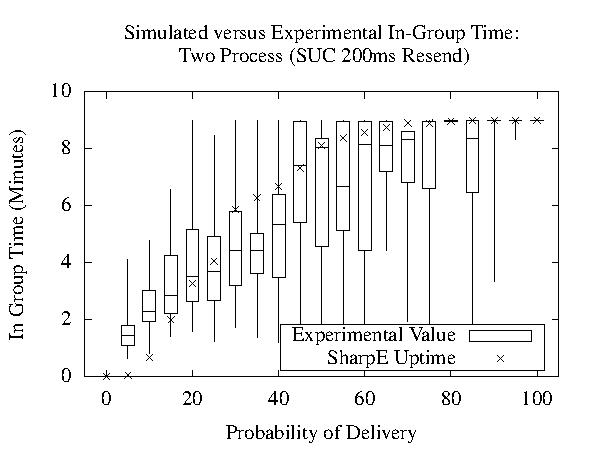
\includegraphics[width=0.75\textwidth]{2NODE-SUC-200-COMPARE.pdf}
    \caption{Comparison of in-group time as collected from the experimental platform and the simulator (2 tick offset between processes).}
    \label{fig:COMPARE-SUC-2NODE-200}
\end{figure}

The race condition between processes during an election is a consideration in the original leader election algorithm, and is an additional factor here.
The simulator provided a parameter to allow the operator to select how closely synchronized the peers were.
The synchronization parameter was the time difference between when each process would search for leaders.
The exchange of messages, particularly during an election, had a tendency to synchronize processes during elections.
Processes could synchronize even if they did not initially begin in a synchronized state. 
The simulation results aligned best for the 100ms resend case with 1 tick (approximately 100ms difference in synchronization between processes) and 2 ticks (approximately 400ms) in the 200ms resend case.


The structure of the Markov Chain assumed that processes enter the election state simultaneously.
This was an appropriate assumption for the real-time system, since the round-robin scheduler synchronized when processes ran their group management modules.
The simulator was set to assume that the synchronization between processes was very tight.
New experimental data was collected for the 4 process, transient partition case.
The collected data is overlaid with the results from the random walker in Figures \ref{fig:COMPARE-SUC-TRANS-RT-128} and \ref{fig:COMPARE-SUC-TRANS-RT-64}.

\begin{figure}[htbp]
    \centering
    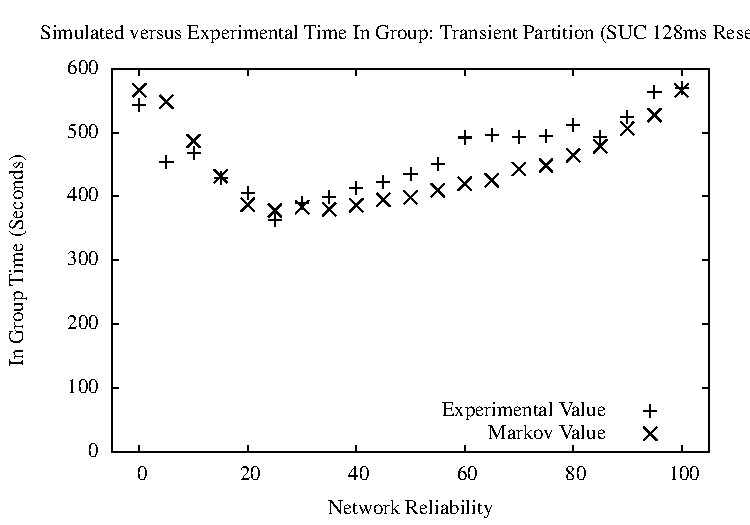
\includegraphics[width=0.75\textwidth]{TRANS-RT-SUC-128-COMPARE.pdf}
    \caption{Comparison of in-group time as collected from the experimental platform and the in-group time from the equivalent Markov chain (128ms between resends).}
    \label{fig:COMPARE-SUC-TRANS-RT-128}
\end{figure}

\begin{figure}[htbp]
    \centering
    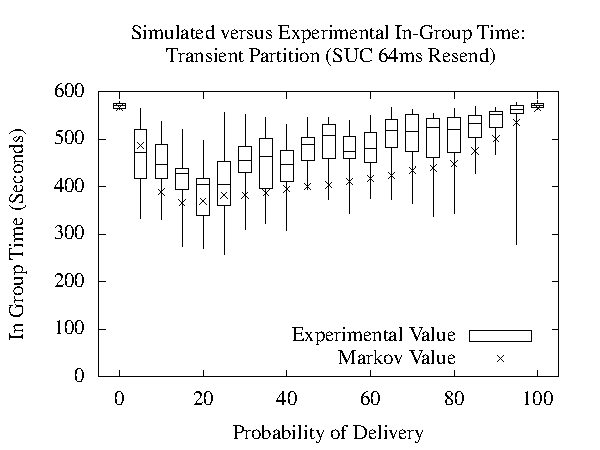
\includegraphics[width=0.75\textwidth]{TRANS-RT-SUC-64-COMPARE.pdf}
    \caption{Comparison of in-group time as collected from the experimental platform and the in-group time from the equivalent Markov chain (64ms between resends).}
    \label{fig:COMPARE-SUC-TRANS-RT-64}
\end{figure}

As a measure of the strength of the model, the correlation between the predicted value was compared.
The average error was also computed for each of the samples taken.
This information is presented in Table \ref{tab:STAT-DATA}.
These results were not sufficient to accurately describe the behavior of the system during fault conditions.
As a result, we sought to refine the analysis of the model in order to get an accurate portrayal of the behavior of the system during faults.

\begin{table}
% increase table row spacing, adjust to taste
\caption{Comparison of collected data compared to Markov chain.}
\label{tab:STAT-DATA}
\centering
% Some packages, such as MDW tools, offer better commands for making tables
% than the plain LaTeX2e tabular which is used here.
\begin{tabular}{|c||c|c|c|}
\hline
Re-send & Correlation & Error \\ \hline
128 & 0.7656 & 11.61\% \\ \hline
64 & 0.8604 & 11.70\% \\ \hline
\end{tabular}
\end{table}
\section{REMARKS}

To ensure the critical infrastructure can safely and reliably provides services to those needing the service, it is necessary to understand how the infrastructure behaves during faults.
Conceptually, using unvetted critical infrastructure, especially when the infrastructure relies heavily on communication, is the same as stepping into an elevator without a safety brake.
Strong analysis of a system's behavior during a failure scenario is paramount to ensuring the safety of those using the infrastructure.

We propose knowledge of the correctness of the operation may be more important than the efficiency of the operation of that critical infrastructure.
Through this work we demonstrate how distributed algorithms can be improved by reasoning about them using information flow security models.
Using these models, one can analyze where the certainty of the system is placed as well as ensuring that the algorithms can be modeled without complete and perfect information of the system.

The models created in this way allow a distributed critical infrastructure system to adjust its behavior, hardening itself against failures.
With this hardening technique, the algorithms used by the system can prevent critical failures that could decrease quality of life for the people using that system.
Subsequent chapters show how information flow methods can be used to determine the memorylessness of aspects of a distributed system, how those aspects can be used to construct a model, and applications of those models.
